\section{Experimental Setup}

We first state our problem, then describe our data, showing all its characteristics. Then, we provide our hypothesis, define the setup, and perform the testing. Finally, we collect and perform data analysis.

\subsection{Problem Statement}

As introduced in the first section of this paper, sorting is a fundamental concept and essential for solving other problems. The content of memory location can change unexpectedly, i.e., faults may happen at any time. Considering this, the main objective of this work is to design experiments to answer the following question: \textit{How are sorting algorithms affected by memory faults?}

\subsection{Variables}

For this experimental study, we assume that the independent and dependent variables are as shown in Table \ref{table-independent-variables} and Table \ref{table-dependent-variables} below:

\begin{table}[H]
    \caption{Independent variables.}
    \begin{center}
    \begin{tabular}{|l|l|}
    \hline
    \textbf{Variable} & \textbf{Description} \\
    \hline
    Probability of failure & Probability of a fault to occur \\
    \hline
    Array size & Size of the array of integers to be sorted \\
    \hline
    Sorting algorithm & Algorithm used to sort the array \\
    \hline
    \end{tabular}
    \label{table-independent-variables}
    \end{center}
\end{table}

\begin{table}[H]
    \caption{Dependent variables.}
    \begin{center}
    \begin{tabular}{|l|l|}
    \hline
    \textbf{Variable} & \textbf{Description} \\
    \hline
    Largest subarray size & Size of the largest sorted subarray produced under the memory fault \\
    \hline
    Percentage of largest subarray size & Percentage of \textit{largest subarray size} related to \textit{array size} independent variable \\
    \hline
    Unordered elements quantity & Quantity of elements out of position after sorting algorithm execution. Adapted of the \\ & \textit{k-unordered sequence} measure of disorder defined in \cite{Ferraro-Petrillo2009} \\
    \hline
    Percentage of unordered elements quantity & Percentage of \textit{unordered elements quantity} related to \textit{array size} independent variable \\
    \hline
    \end{tabular}
    \label{table-dependent-variables}
    \end{center}
\end{table}

\subsection{Hypothesis}

The set of hypothesis defined to test and draw some conclusions about this experiment are listed below. The confidence degree defined for hypothesis testing was 95\% ($\alpha = 0.05$ and $\alpha - 1 = 0.95$).

\begin{itemize}
    \item \textbf{Hypothesis 1:} For a given probability of failure and array size, tested algorithms will produce a different percentage of unordered elements quantity.
    \item \textbf{Hypothesis 2:} For a given probability of failure and array size, tested algorithms will produce a different percentage of the largest subarray size.
    \item \textbf{Hypothesis 3:} For each algorithm, the array size and probability of failure have a significative impact on the percentage of unordered elements quantity.
    \item \textbf{Hypothesis 4:} For each algorithm, the array size and probability of failure have a significative impact on the percentage of the largest subarray size.
\end{itemize}

% \setcounter{hyp}{-1}
% \begin{hyp}[Test hypothesis] \label{hyp:a}There is no difference in memory faults between tested algorithms.\end{hyp}
% \begin{hyp} \label{hyp:b}There are differences in memory faults between tested algorithms. \end{hyp}
% \begin{hyp} \label{hyp:c} An algorithm is better than others considering all dependent variables. \end{hyp}

% \begin{hyp} \label{hyp:d} ... \end{hyp}

\subsection{Dataset}

To conduct the proposed study, we define the values of the independent variables, as shown in Table \ref{table-independent-variables-values}:

\begin{table}[H]
    \caption{Values of the independent variables.}
    \begin{center}
    \begin{tabular}{|c|c|}
    \hline
    \textbf{Variable} & \textbf{Values} \\
    \hline
    Probability of failure & 1\%, 2\% and 5\% \\
    \hline
    Array size & 100, 1000 and 10000 \\
    \hline
    Sorting algorithm & Bubblesort, Quicksort, Mergesort and Insertion sort \\
    \hline
    \end{tabular}
    \label{table-independent-variables-values}
    \end{center}
\end{table}

Based on these variables, we ran an existing script \textit{gen.py} to produce input files. We define that our sample was composed by 30 input files for a given combination of the probability of failure and array size. So, considering this, we ran 30 times for each combination of these independent variables, producing 30 inputs, totalizing 270 files. Figure \ref{fig-input-file-example} shows an example of produced input files:

% \begin{itemize}
%     \item A script that generates input files;
%     \item Four files, one for each of those algorithms: quicksort, bubblesort, insertion sort, and mergesort, that are used to sorting the input data;
% \end{itemize}

\begin{verbbox}[\mbox{}]
0.01 100 9 48 37 6 26 7 24 44 17 50 48 30 49 33 22 13 42 29 39 13 19 13 9 28 
34 1 33 27 14 45 48 40 11 17 6 50 9 44 20 16 37 45 23 14 38 29 10 49 44 46 35
45 15 2 22 1 46 40 8 48 23 23 32 35 3 15 8 36 17 24 27 48 28 5 28 50 44 4 25 
6 9 1 11 44 26 50 44 12 7 20 30 20 37 20 6 8 13 15 20 49
\end{verbbox}

\begin{figure}[H]
    \centering
    \fbox{
    \theverbbox
    }
    \caption{Example of input file.}
    \label{fig-input-file-example}
\end{figure}

The input data shown in the Figure \ref{fig-input-file-example} is divided as follows:

\begin{itemize}
    \item \textit{Probability of Failure}: the first number of the sequence (\texttt{0.01}) is the probability of memory failure when sorting;
    \item \textit{Sequence size}: the second number (\texttt{100}) means the size of the integers sequence used by sorting;
    \item \textit{Sequence}: the rest of the numbers indicates the sequence itself.
\end{itemize}

With this input data, we ran, for each one of these, all four algorithms considered in this study. The sorting algorithms used already existed. For example, using all 270 input files, we ran bubblesort, creating 270 output files, and so on for the other algorithms. At the end of executions, we get a total of 1080 output files. An output file look like shown in Figure \ref{fig-output-file-example}:

% We run 1000 times each algorithm with each file listed in Table \ref{table-input-data} below. We chose this number of executions to reduce possible noise in the generated data. Table \ref{table-input-data} shows 9 different input files with its sequence sizes and probabilities of failure. Plus, the number of executions and each sorting algorithm.

% For example, Input A showed in that table with its characteristics was executed 1000 times for each algorithm -  bubblesort, quicksort, mergesort, and insertion sort - totalizing 4000 executions.

% \begin{table}[H]
%     \caption{Generated input data.}
%     \begin{center}
%     \begin{tabular}{|c|c|c|c|c|}
%     \hline
%     \textbf{Input} & \textbf{Sequence Size} & \textbf{Probability of Failure} & \textbf{Executions} & \textbf{Algorithm} \\ 
%     \hline
%     \multirow{4}{*}{Input A} & \multirow{4}{*}{100} & \multirow{4}{*}{1\%} & \multirow{4}{*}{1000} & Bubblesort \\ 
%     & & & & Quicksort \\
%     & & & & Mergesort \\
%     & & & & Insertion Sort \\
%     \hline
%     \multirow{4}{*}{Input B} & \multirow{4}{*}{100} & \multirow{4}{*}{2\%} & \multirow{4}{*}{1000} & Bubblesort \\ 
%     & & & & Quicksort \\
%     & & & & Mergesort \\
%     & & & & Insertion Sort \\
%     \hline
%     \multirow{4}{*}{Input C} & \multirow{4}{*}{100} & \multirow{4}{*}{5\%} & \multirow{4}{*}{1000} & Bubblesort \\ 
%     & & & & Quicksort \\
%     & & & & Mergesort \\
%     & & & & Insertion Sort \\
%     \hline
%     \multirow{4}{*}{Input D} & \multirow{4}{*}{1000} & \multirow{4}{*}{1\%} & \multirow{4}{*}{1000} & Bubblesort \\ 
%     & & & & Quicksort \\
%     & & & & Mergesort \\
%     & & & & Insertion Sort \\
%     \hline
%     \multirow{4}{*}{Input E} & \multirow{4}{*}{1000} & \multirow{4}{*}{2\%} & \multirow{4}{*}{1000} & Bubblesort \\ 
%     & & & & Quicksort \\
%     & & & & Mergesort \\
%     & & & & Insertion Sort \\
%     \hline
%     \multirow{4}{*}{Input F} & \multirow{4}{*}{1000} & \multirow{4}{*}{5\%} & \multirow{4}{*}{1000} & Bubblesort \\ 
%     & & & & Quicksort \\
%     & & & & Mergesort \\
%     & & & & Insertion Sort \\
%     \hline
%     \multirow{4}{*}{Input G} & \multirow{4}{*}{10000} & \multirow{4}{*}{1\%} & \multirow{4}{*}{1000} & Bubblesort \\ 
%     & & & & Quicksort \\
%     & & & & Mergesort \\
%     & & & & Insertion Sort \\
%     \hline
%     \multirow{4}{*}{Input H} & \multirow{4}{*}{10000} & \multirow{4}{*}{2\%} & \multirow{4}{*}{1000} & Bubblesort \\ 
%     & & & & Quicksort \\
%     & & & & Mergesort \\
%     & & & & Insertion Sort \\
%     \hline
%     \multirow{4}{*}{Input I} & \multirow{4}{*}{10000} & \multirow{4}{*}{5\%} & \multirow{4}{*}{1000} & Bubblesort \\ 
%     & & & & Quicksort \\
%     & & & & Mergesort \\
%     & & & & Insertion Sort \\
%     \hline
%     \end{tabular}
%     \label{table-input-data}
%     \end{center}
% \end{table}

% Each execution generates an output file. Then, we generate 4000 outputs for each combination of sequence size, and the probability of failure, totalizing 36000 files. Figure \ref{fig-output-file-example} shows an output file.

\begin{verbbox}[\mbox{}]
[1]  9 48 37 6 26 7 24 44 17 50 48 30 49 33 22 13 42 29 39 13 19 13 9 28 34 1
33 27 14 45 48 40 11 17 6 50 9 44 20 16 37 45 23 14 38 29 10 49 44 46 35 45  
15 2 22 1 46 40 8 48 23 23 32 35 3 15 8 36 17 24 27 48 28 5 28 50 44 4 25 6 9
1 11 44 26 50 44 12 7 20 30 20 37 20 6 8 13 15 20 49
[2]  1 1 1 2 3 4 5 6 6 6 6 7 7 8 8 8 9 9 9 9 10 11 11 12 13 13 13 13 14 14 15 
15 15 16 17 17 17 19 20 20 20 20 22 22 23 23 23 24 24 25 26 26 27 27 28 28 28 
29 29 30 30 32 33 33 34 35 35 36 37 37 37 38 39 40 40 42 44 44 44 44 44 44 20 
45 45 45 46 46 48 48 48 48 48 49 49 50 49 50 50 50
[3]  1 1 1 2 3 4 5 6 6 6 6 7 7 8 8 8 9 9 9 9 10 11 11 12 13 13 13 13 14 14 15 
15 15 16 17 17 17 19 20 20 20 20 20 22 22 23 23 23 24 24 25 26 26 27 27 28 28 
28 29 29 30 30 32 33 33 34 35 35 36 37 37 37 38 39 40 40 42 44 44 44 44 44 44 
45 45 45 46 46 48 48 48 48 48 49 49 49 50 50 50 50
[4]  82
\end{verbbox}
    
\begin{figure}[H]
    \centering
    \fbox{
    \theverbbox
    }
    \caption{Example of output file.}
    \label{fig-output-file-example}
\end{figure}

The output file gives four essential data, as enumerated below:
\begin{itemize}
    \item \textit{[1]}: the original sequence of integers contained in the input file;
    \item \textit{[2]}: the sequence processed by the sorting algorithm under the memory fault model;
    \item \textit{[3]}: the sequence sorted correctlty;
    \item \textit{[4]}: the size of the largest sorted subsequence in [2]. This number can be interpreted as the quality of sorting. As higher, most successful was the sorting operation.
\end{itemize}

After generating the dataset, we developed a Python script that reads the 1080 output files and produces a single CSV file (first lines showed in Figure \ref{fig-output-csv-file-example} below), containing the following columns:
\begin{itemize}
    \item \textit{algorithm}: the algorithm used to sort the array;
    \item \textit{probability\_of\_failure}: the probability of failure used when sorting;
    \item \textit{size\_of\_array}: the size of the array to be sorted;
    \item \textit{largest\_sorted\_subarray}: the largest sorted subarray after sorting;
    \item \textit{k\_unordered\_sequence}: number of unordered sequence after sorting.
    \item \textit{percentage\_k\_unordered}: percentage of unordered sequence after sorting related to original array;
    \item \textit{percentage\_largest\_sorted\_subarray}: percentage of largest sorted subarray after sorting related to original array.
\end{itemize}

\begin{verbbox}[\mbox{}]
algorithm;probability_of_failure;size_of_array;largest_sorted_subarray;
k_unordered_sequence;percentage_k_unordered;
percentage_largest_sorted_subarray
quick;0.01;100;35;4;4.00;35.00
quick;0.01;100;36;8;8.00;36.00
quick;0.01;100;31;5;5.00;31.00
quick;0.01;100;20;6;6.00;20.00
quick;0.01;100;31;5;5.00;31.00
\end{verbbox}
        
\begin{figure}[H]
    \centering
    \fbox{
    \theverbbox
    }
    \caption{Example of output CSV file.}
    \label{fig-output-csv-file-example}
\end{figure}

We use Python libraries to make data analysis and plot graphs. These libraries were:
\begin{itemize}
    \item \textit{Pandas\footnote{https://pandas.pydata.org}}: open source library providing data structures and data analysis tools;
    \item \textit{NumPy\footnote{https://numpy.org}}: library for scientific computing with Python;
    \item \textit{SciPy\footnote{https://www.scipy.org}}: ecosystem of open-source software for mathematics, science, and engineering;
    \item \textit{StatsModels\footnote{https://www.statsmodels.org}}: module that provides classes and functions for the estimation of many different statistical models, as well as for conducting statistical tests, and statistical data exploration;
    \item \textit{Matplotlib\footnote{https://matplotlib.org}}: plotting library;
    \item \textit{Seaborn\footnote{https://seaborn.pydata.org}}: data visualization library based on matplotlib.
\end{itemize}

% \subsection{Data Analysis}

% In this section, we describe our data and the statistic tests used to test the hypothesis showed before.

% \subsubsection{Exploratory Data Analysis (EDA)}

% Based on the output files generated before, our starting point was to test if the dataset had a normal distribution. To achieve this, we use Shapiro-Wilk normality test. After we run these tests, only the distribution related to the dependent variable \textit{unordered elements size} was considered normal. Figure \ref{fig-distribution-graph} shows an example of this distribution. In these graphs, the red vertical line means the mean, and the blue vertical line means the median. The distributions were normal in all combinations of independent variables for dependent variable \textit{unordered elements size}.

% \begin{figure}[H]
%     \centering
%      \begin{subfigure}{.5\textwidth}
%      \centering
%      \frame{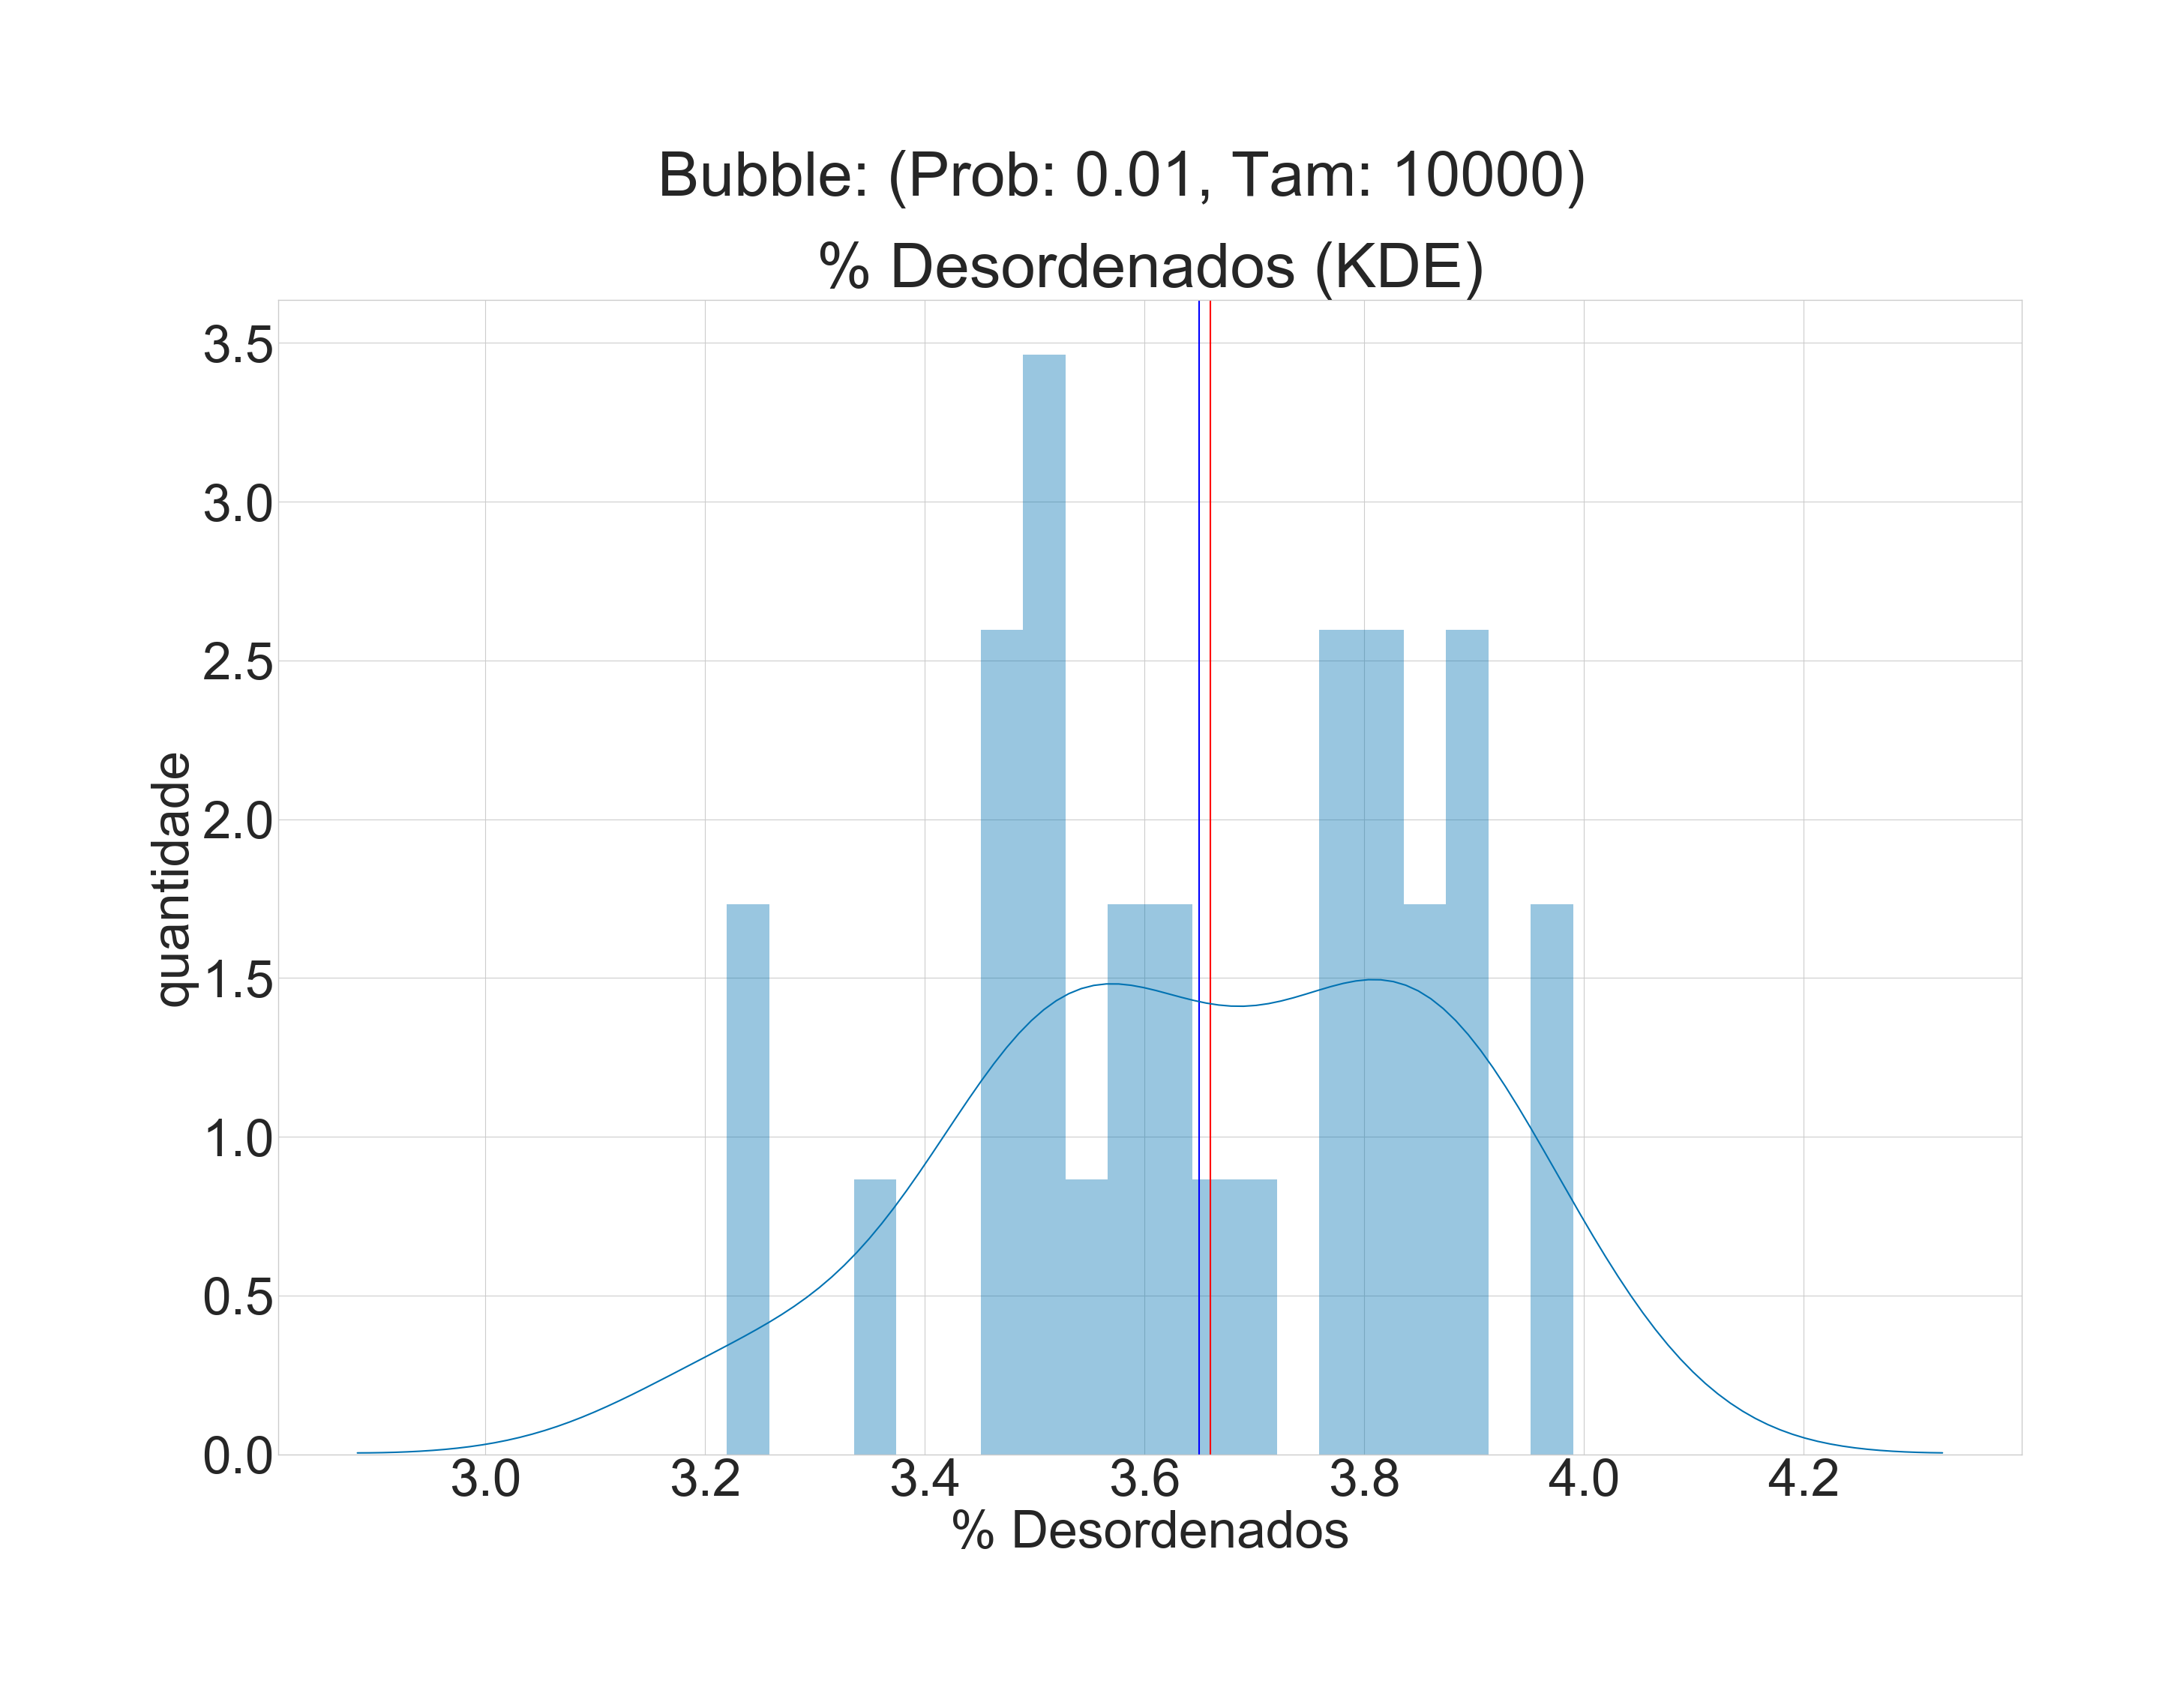
\includegraphics[scale=0.12]{figures/0_01_10000_Bubble_distribution_graph}}
%      \textsf{\caption[Distribution Graph for bubblesort.]{Distribution Graph for bubblesort.\label{fig-dist-bubble-001-100}}}
%      \end{subfigure}%
%      \begin{subfigure}{.5\textwidth}
%      \centering
%      \frame{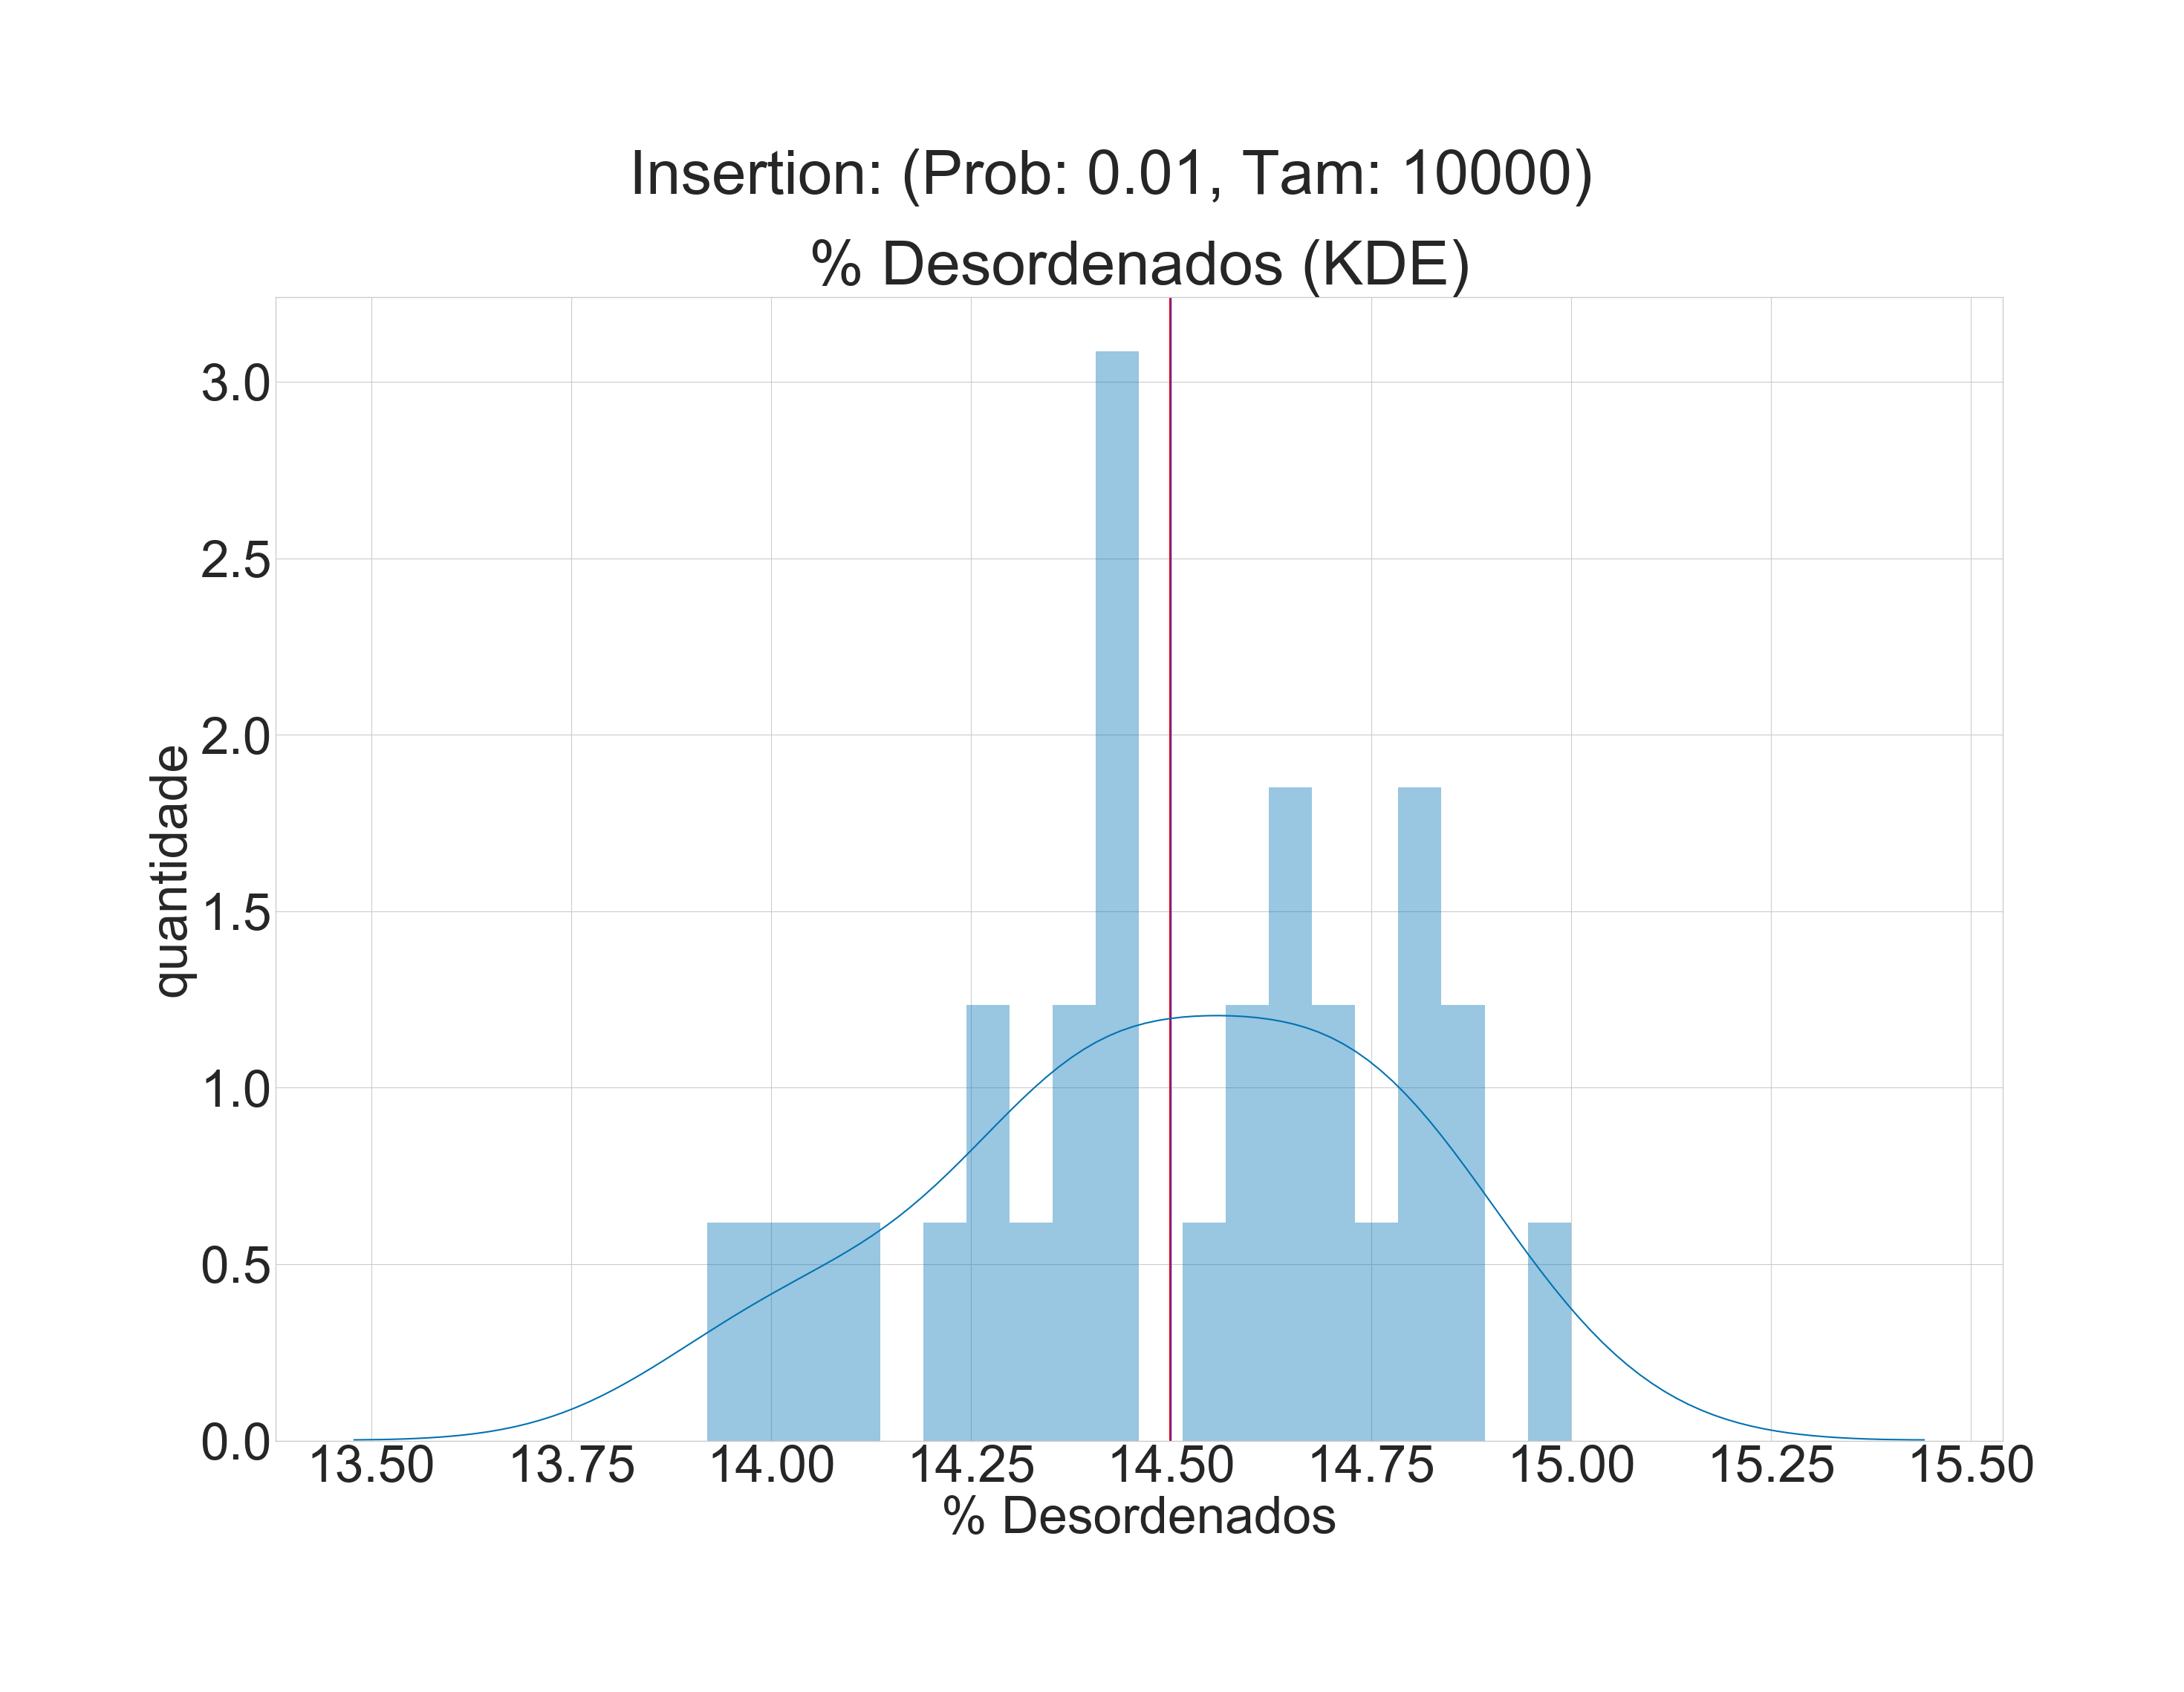
\includegraphics[scale=0.12]{figures/0_01_10000_Insertion_distribution_graph.png}}
%      \textsf{\caption[Distribution Graph for insertion sort.]{Distribution Graph for insertion sort.\label{fig-dist-insertion-001-100}}}
%      \end{subfigure}
%      \begin{subfigure}{.5\textwidth}
%      \centering
%      \frame{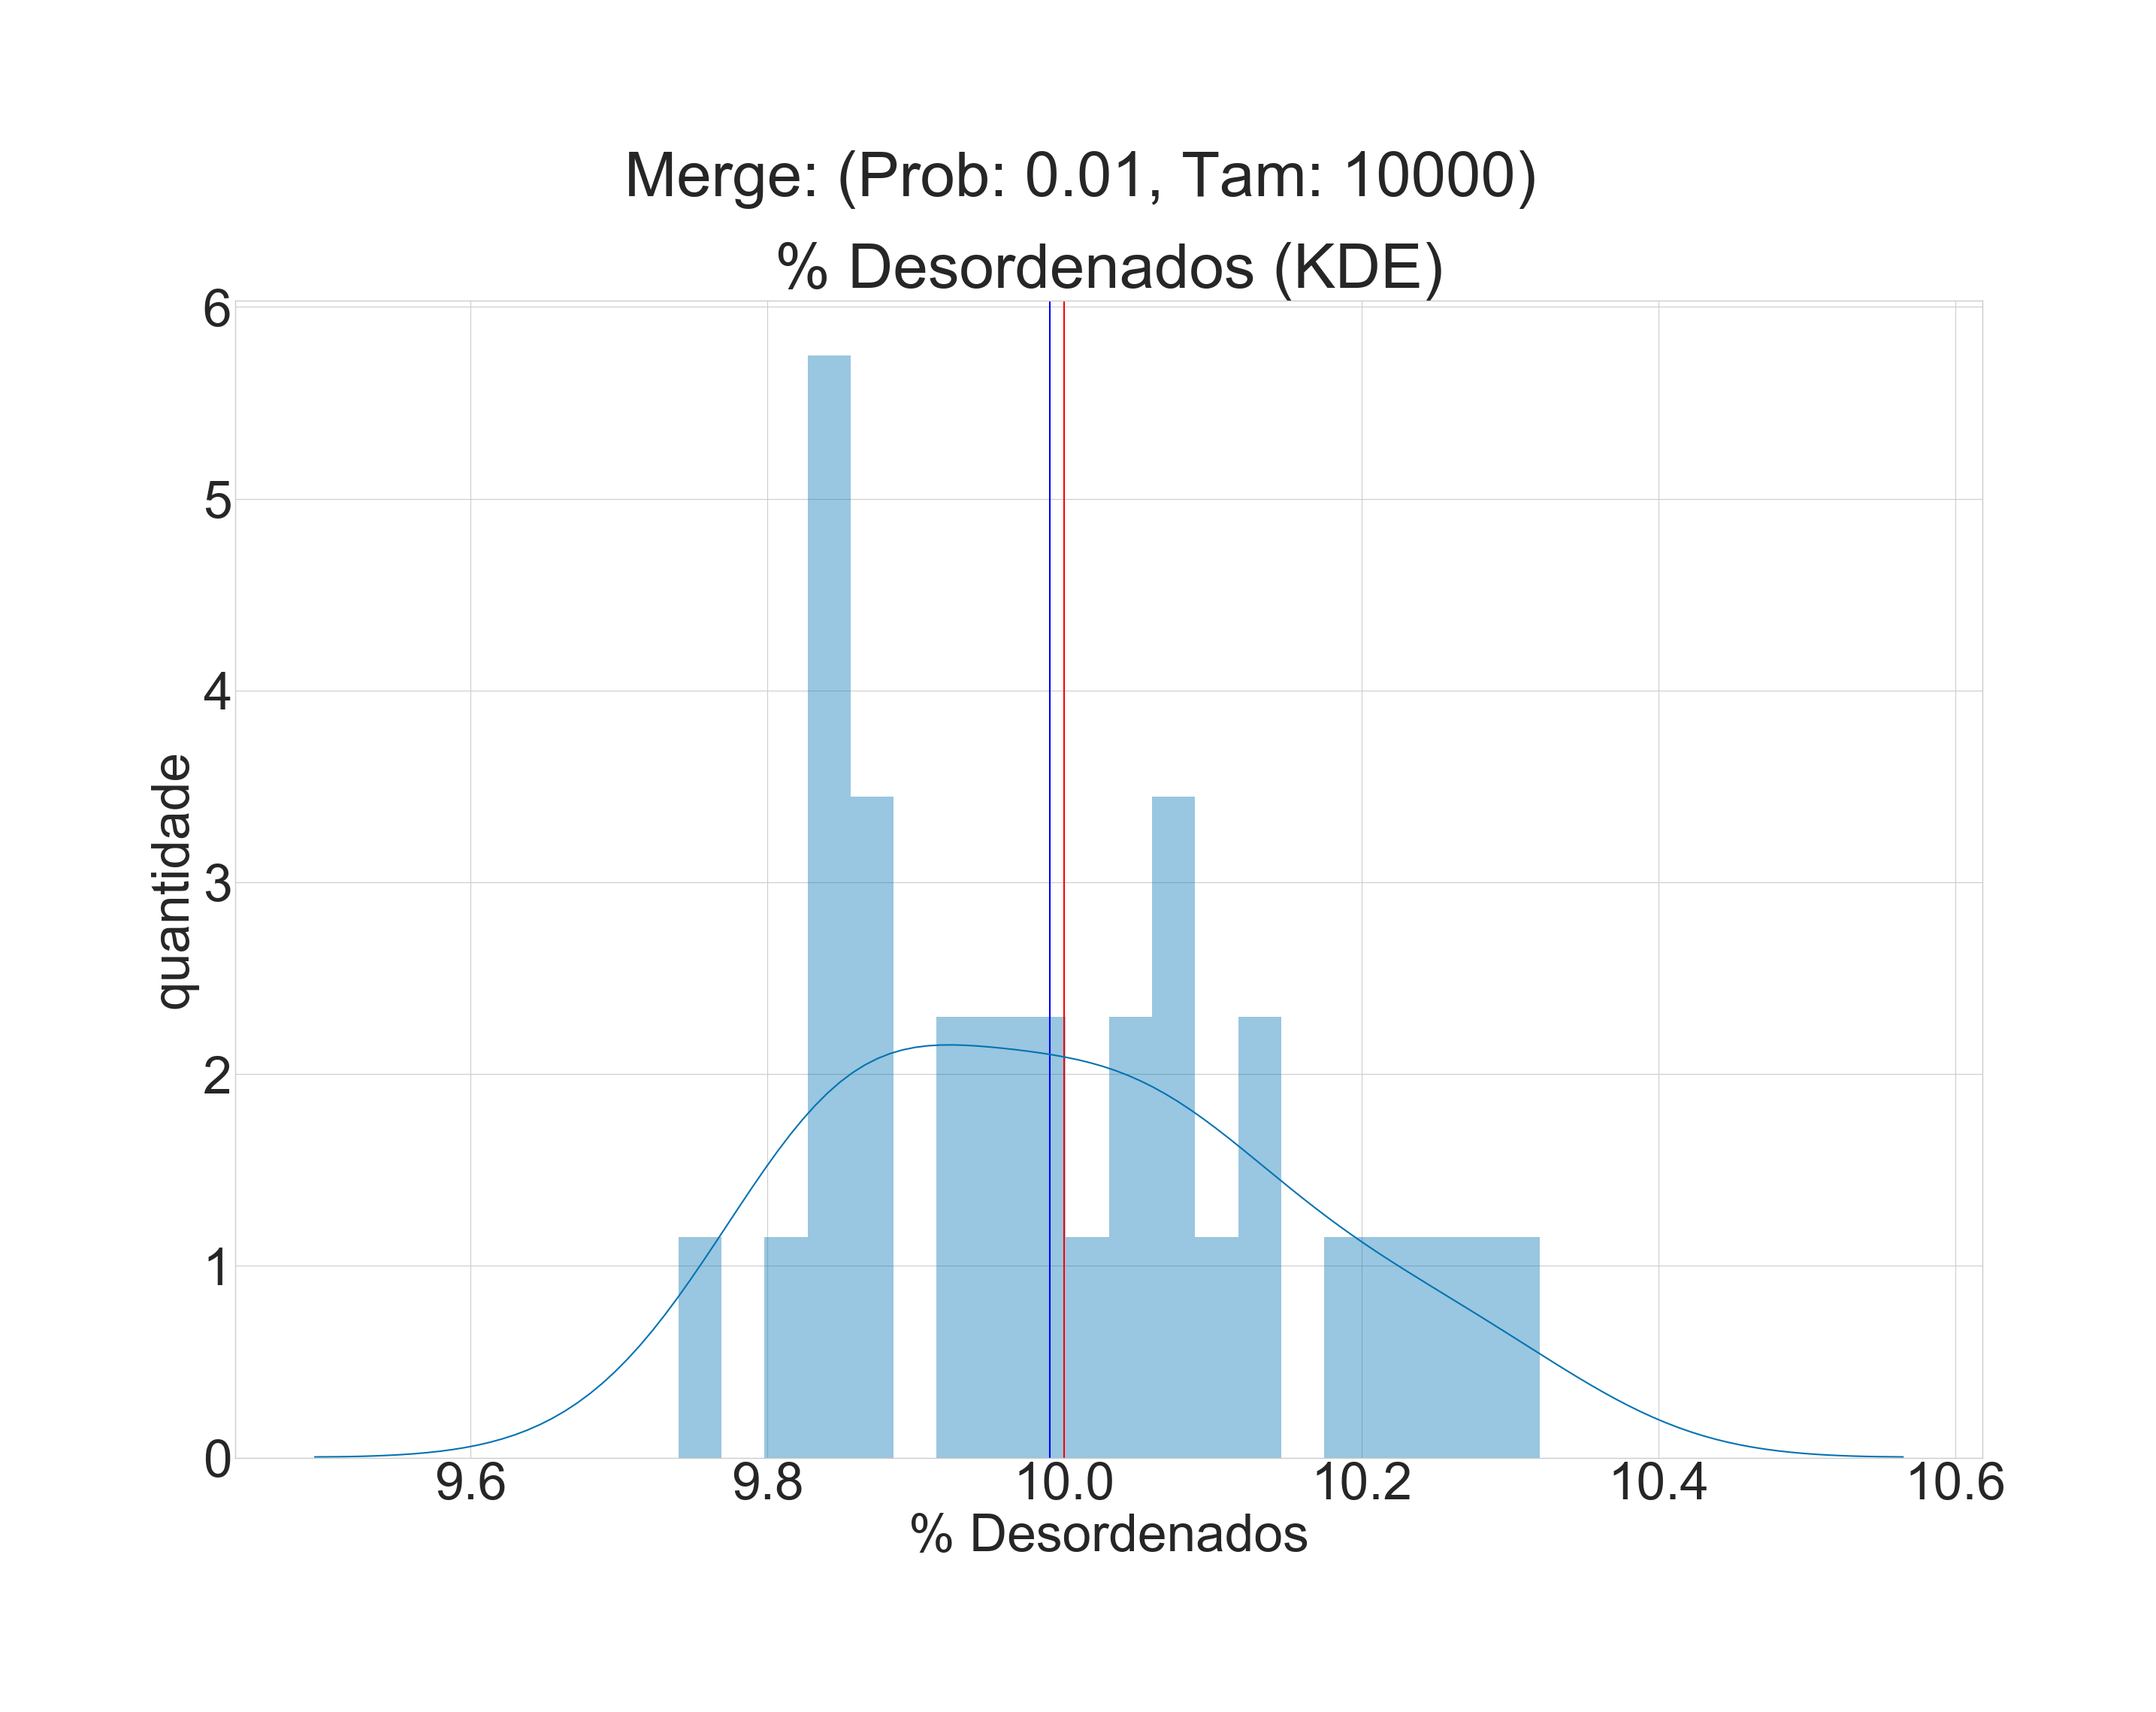
\includegraphics[scale=0.12]{figures/0_01_10000_Merge_distribution_graph.png}}
%      \textsf{\caption[Distribution Graph for mergesort.]{Distribution Graph for mergesort.\label{fig-dist-merge-001-100}}}
%      \end{subfigure}%
%      \begin{subfigure}{.5\textwidth}
%      \centering
%      \frame{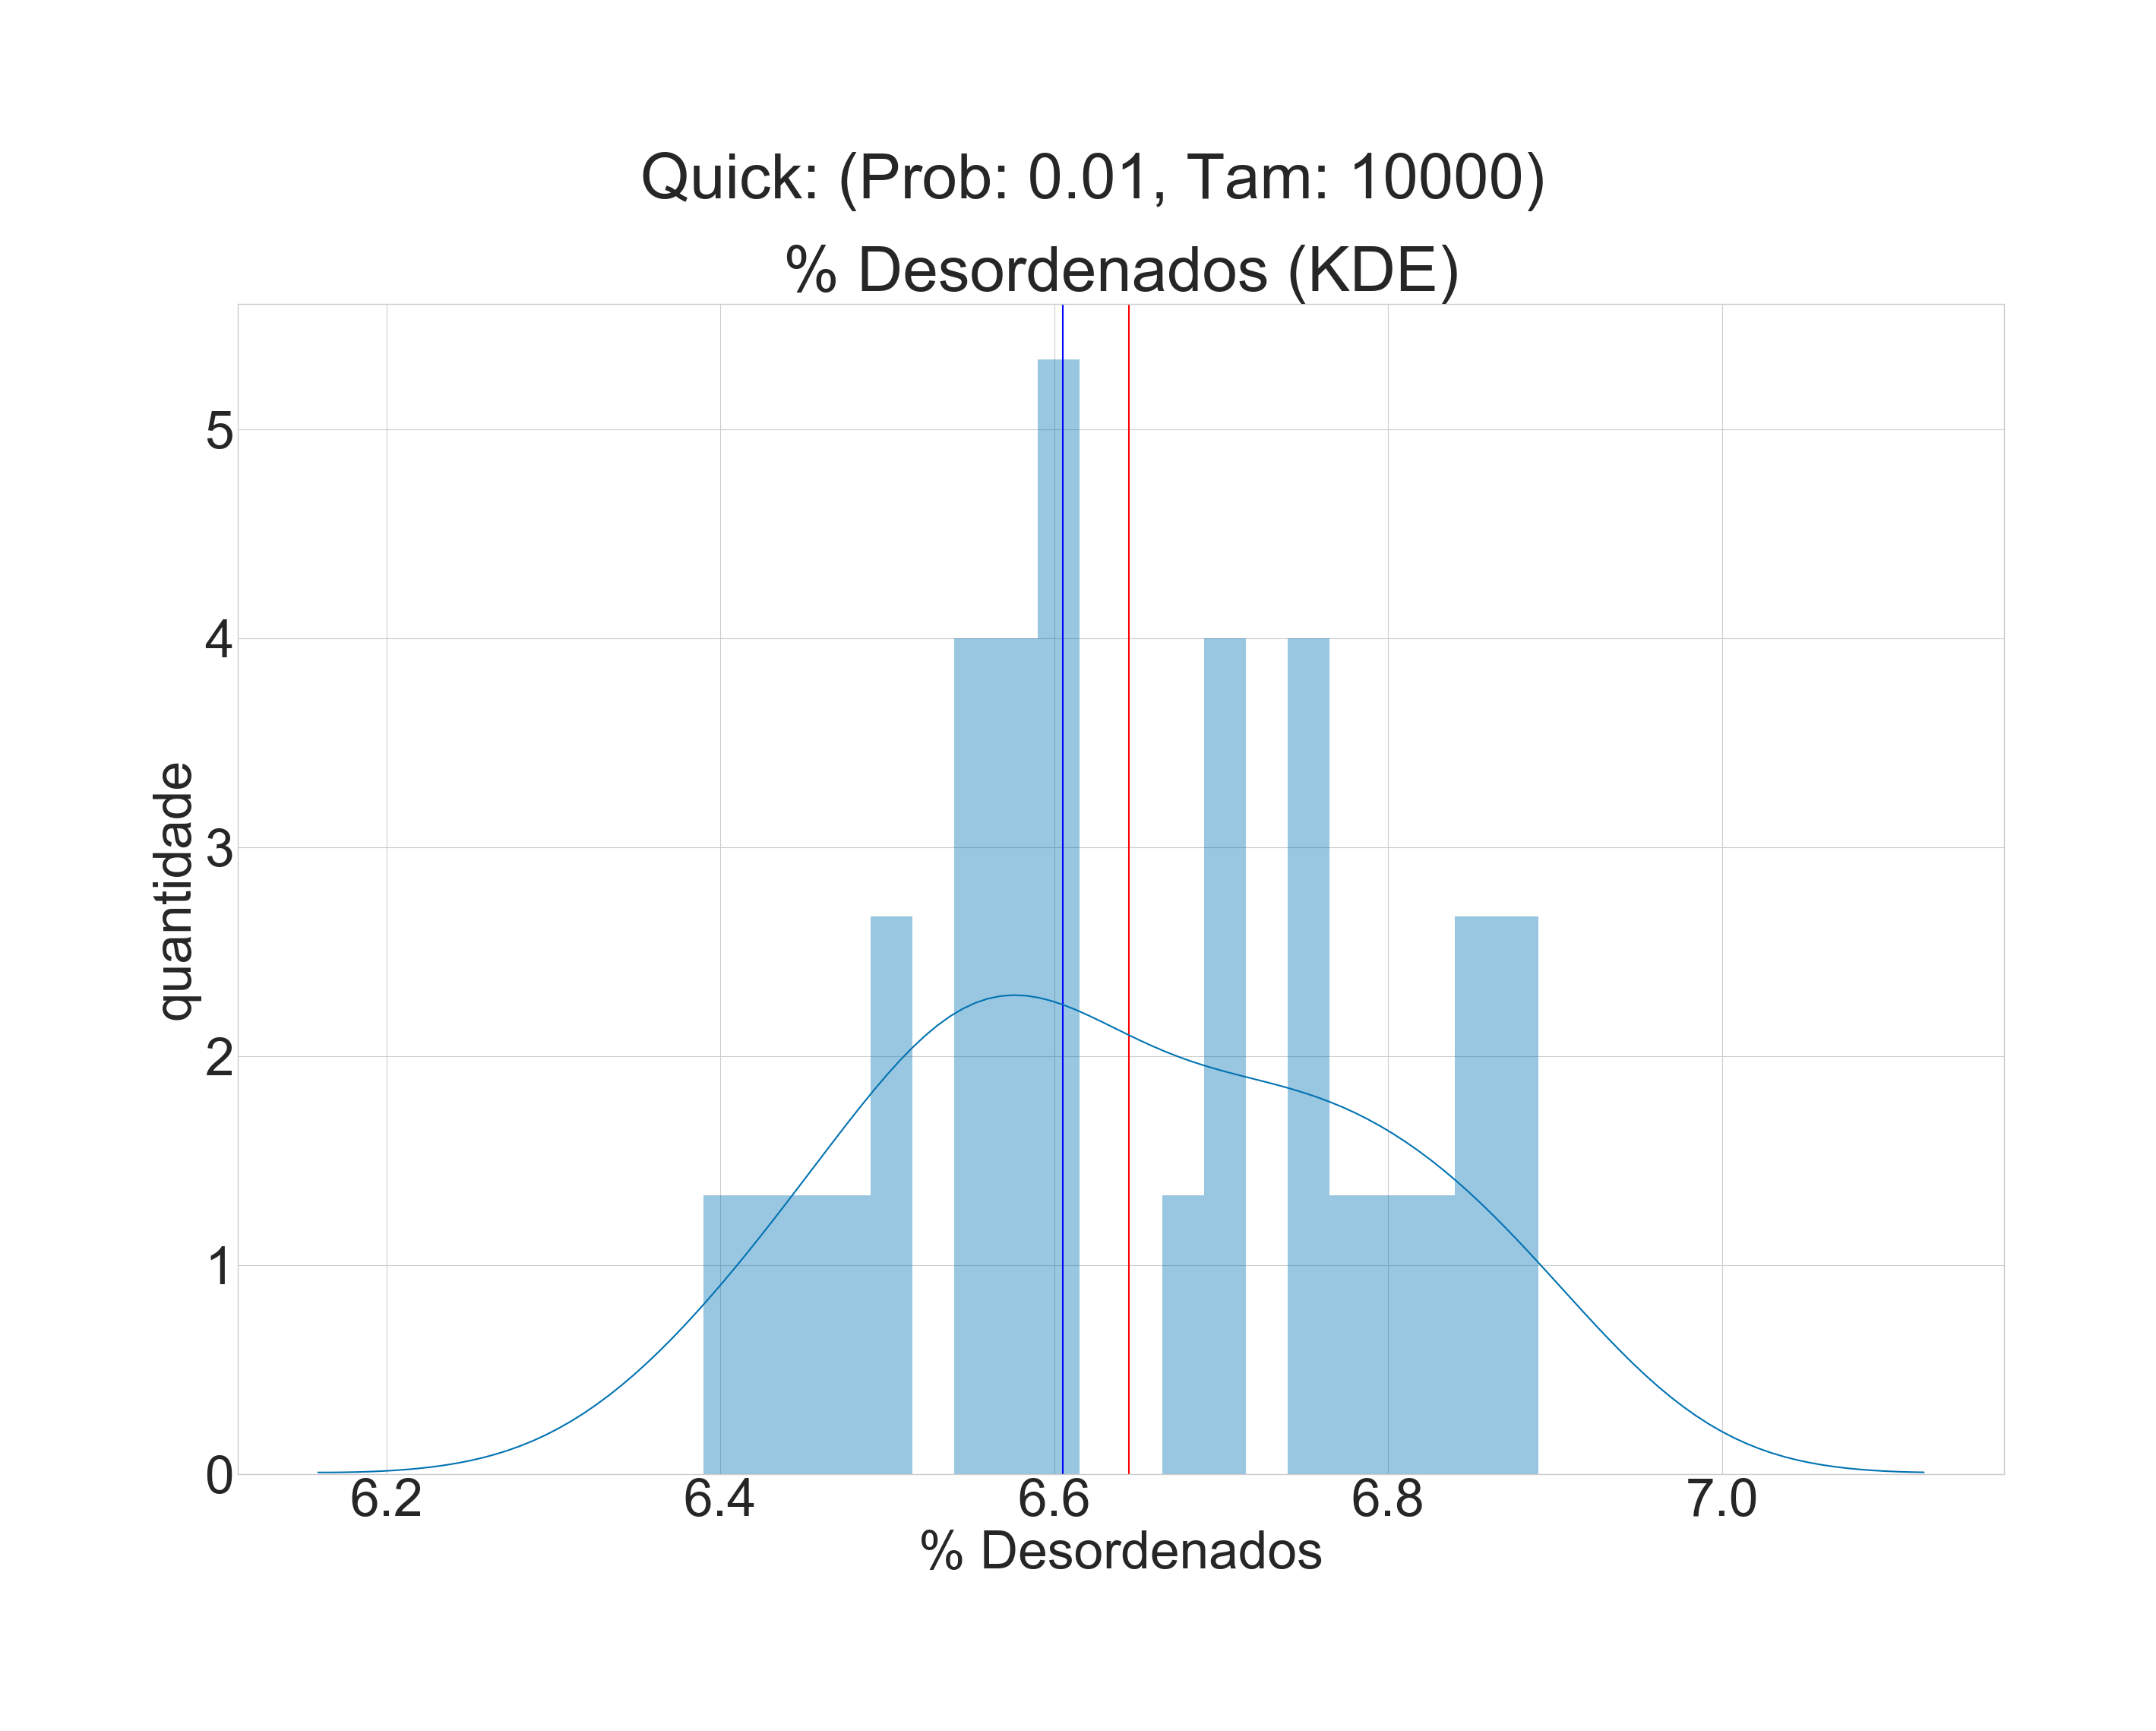
\includegraphics[scale=0.12]{figures/0_01_10000_Quick_distribution_graph.png}}
%      \textsf{\caption[Distribution Graph for quicksort.]{Distribution Graph for quicksort.\label{fig-dist-quick-001-100}}}
%      \end{subfigure}
%      \caption{Distribution graph for a probability failure of 1\% and a sequence size of 10000.}
%     \label{fig-distribution-graph}
% \end{figure}

% Q-Q plot shows that how much more blue points close to the red line, most normal is the distribution. Figure \ref{fig-qqplot} below presents this graph for a probability failure of 1\% and a sequence size of 10000 for considered sorting algorithms.

% \begin{figure}[H]
%     \centering
%     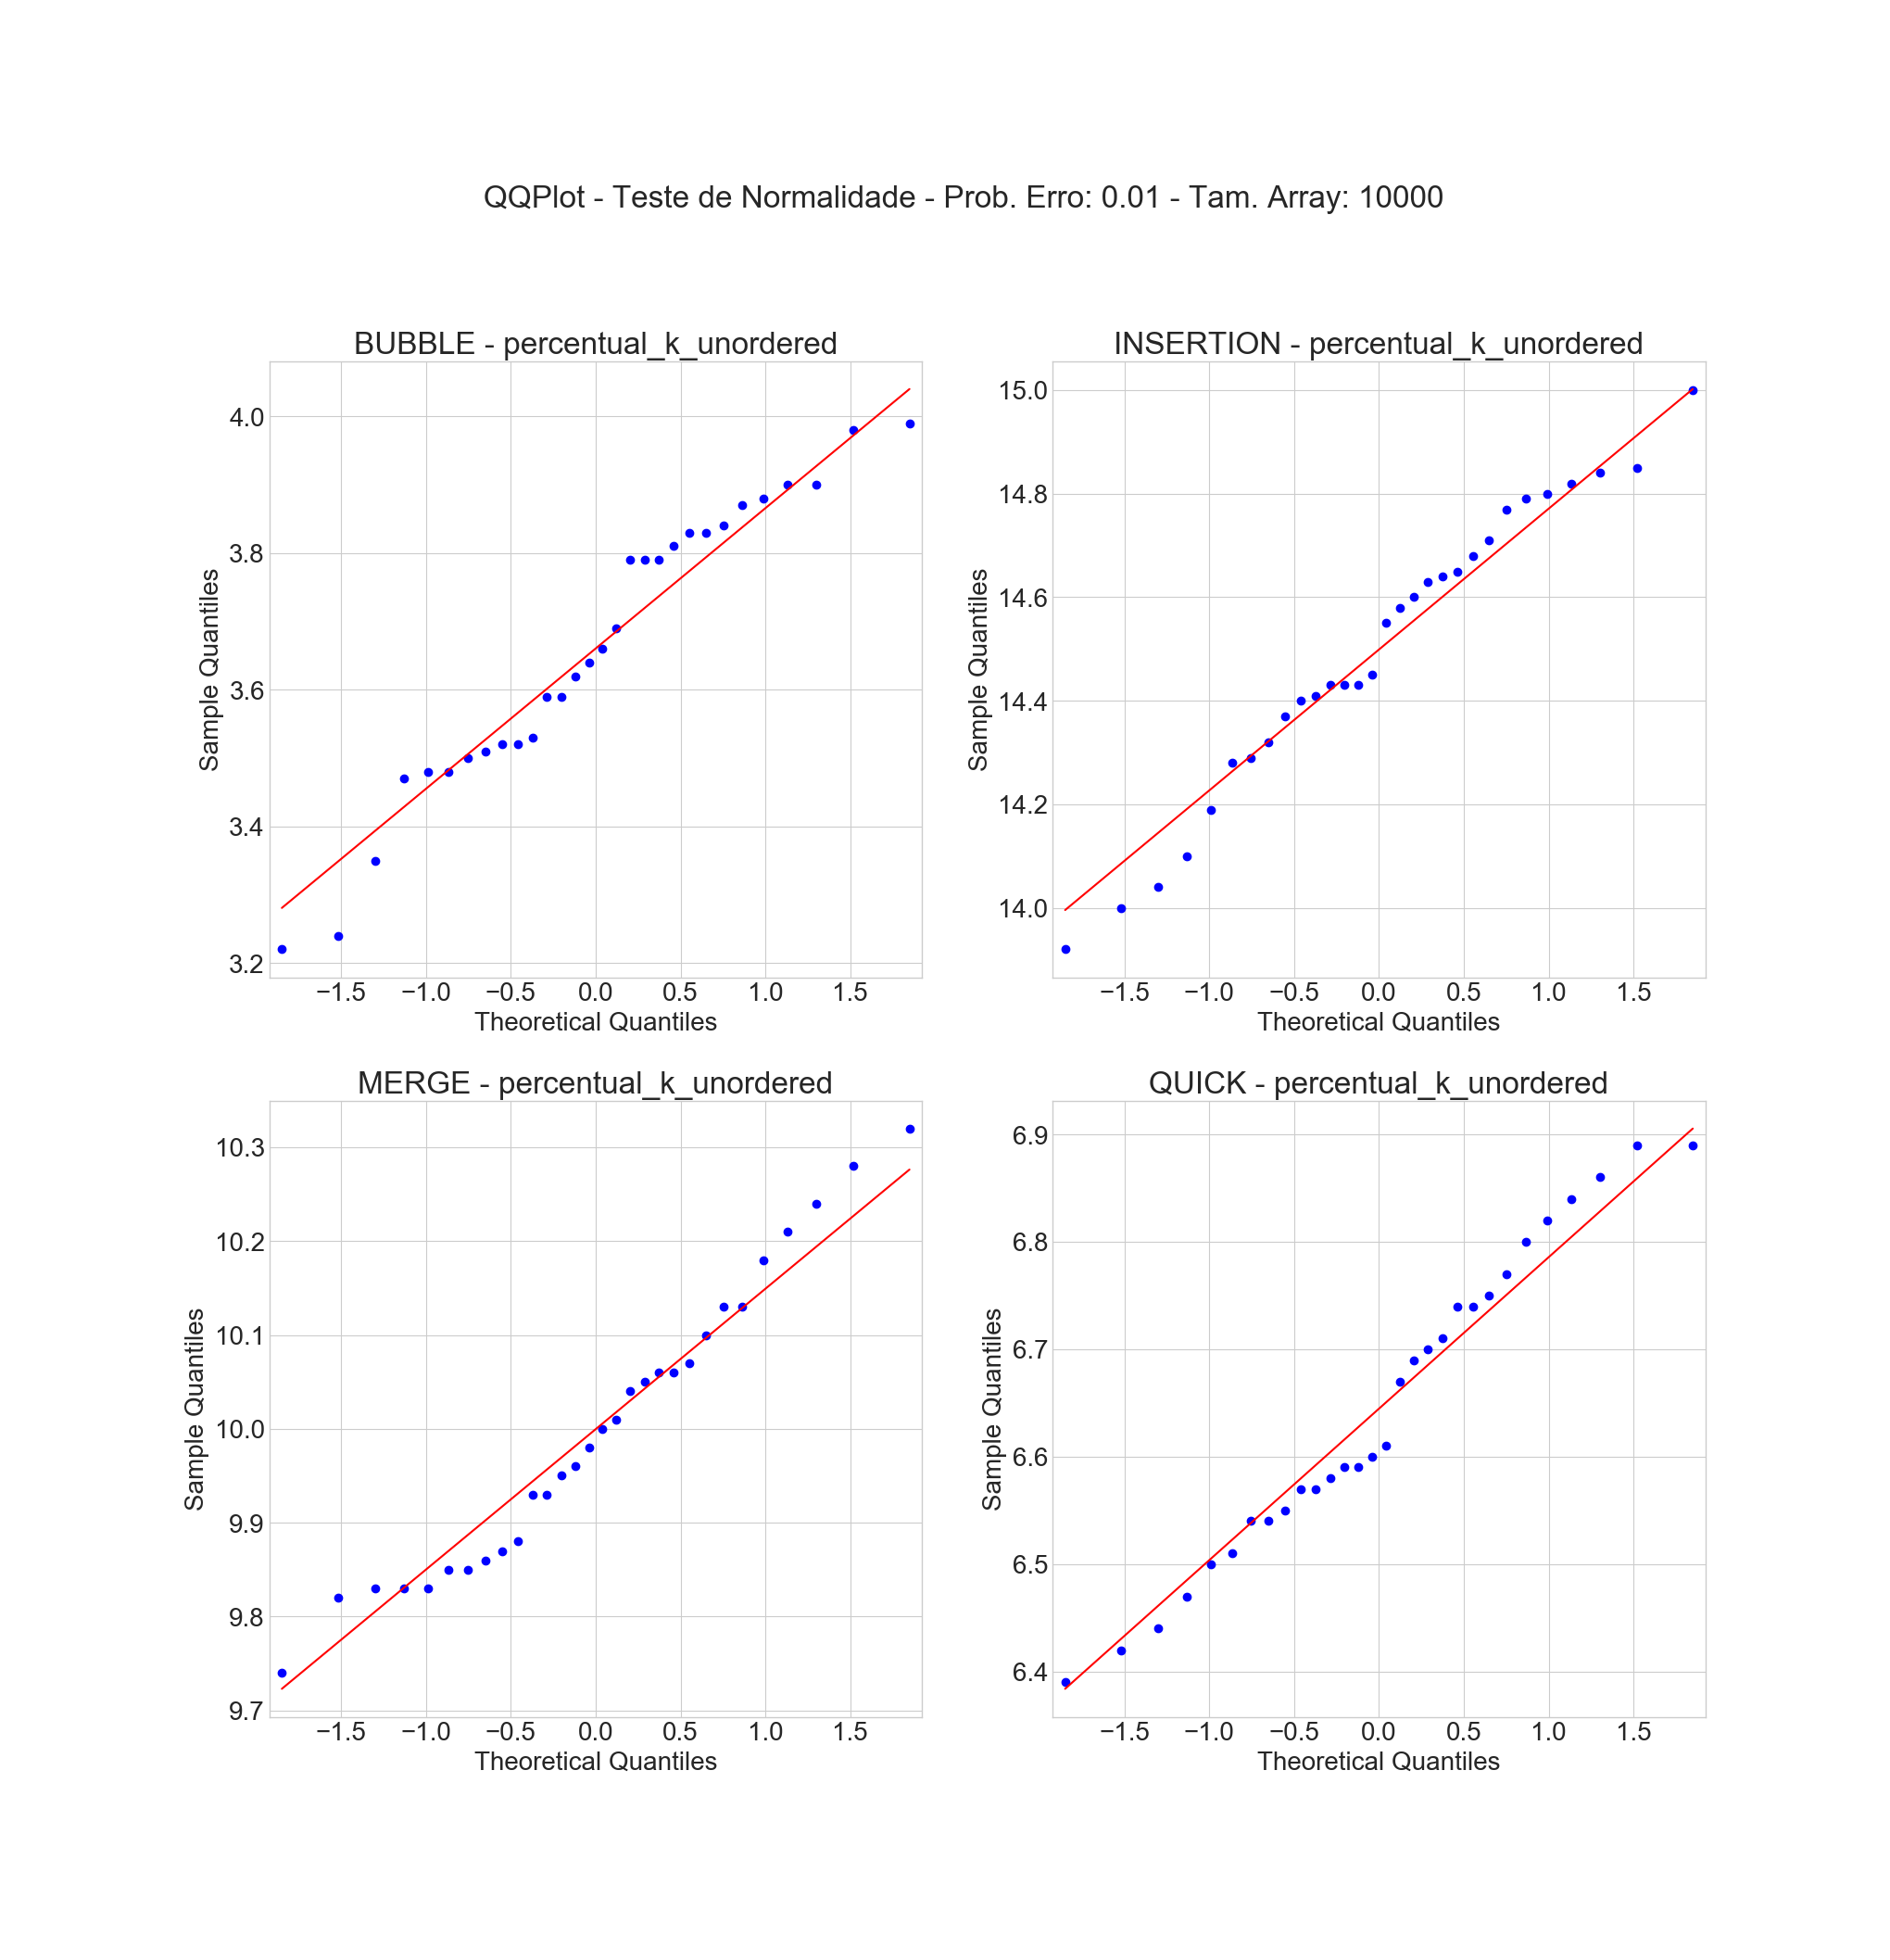
\includegraphics[scale=0.37]{figures/anova_prob_0_01_tam_10000_DESORDENADOS_PERCENTUAL.png}
%     \textsf{\caption[Q-Q plot showing normal distribution for a probability failure of 1\% and a sequence size of 10000.]{Q-Q plot showing normal distribution for a probability failure of 1\% and a sequence size of 10000.\label{fig-qqplot}}}
%  \end{figure}

\subsection{Conclusions}

